% Build: tectonic paper/main.tex
\documentclass[11pt]{article}
\usepackage[margin=1in]{geometry}
\usepackage{amsmath,amssymb,array,booktabs,float,graphicx,natbib,xcolor}
\usepackage{flafter}  % a table or figure never appears before the text that introduces it
\emergencystretch=2em  % no line runs into the margin for want of a break
\definecolor{linkblue}{RGB}{0,51,153}
\usepackage[colorlinks=true,allcolors=linkblue]{hyperref}
\newcommand{\todo}[1]{\textcolor{red}{[#1]}}
\newcommand{\para}[1]{\paragraph{#1}}
% Clickable DOIs in the reference list (plainnat only \providecommand's \doi, so this one is used).
\newcommand{\doi}[1]{\href{https://doi.org/#1}{doi:\,#1}}
\title{Take a Deep Breath?\\
Relaxation Prompts Calm Language-Model Replies\\
With or Without Prior Anxiety Induction}
\author{Jiajun Ma}
\date{November 2026}
\begin{document}
\maketitle
\begin{abstract}
Language models are now used in mental-health support, and studies borrow clinical methods to make a
model anxious and calm it again: traumatic narratives raise its score on an anxiety questionnaire,
and relaxation exercises lower it.
If the exercise undoes what the narrative induced, such prompts could steady a model in difficult
conversations.
The published tests, however, give the exercise only after a narrative, and compare the score with
the one before the narrative or with the score after neutral filler text.
Neither comparison can tell an exercise that reverses what the narrative induced from calm text that
calms a reply whatever came before it.
In seven open-weight models we add a reading of the activations along an anxious-versus-calm
direction, taken while the model writes its reply, and a version of every conversation with a neutral
passage in place of the narrative.
After a narrative, relaxation recovers more of the rise than filler in all seven models, on the
questionnaire and in the activations.
Without a narrative, it still lowers the activation reading by 0.60 to 2.17 standard deviations in
six models, and its advantage over filler is nearly the same: the narrative adds 0.14 standard
deviations on average (95\% interval $-0.16$ to 0.43), confirmed in one model of seven.
A drop after relaxation is therefore not evidence that the exercise regulates an induced state.
Nor do our results rule such a state out, because the activation reading follows the wording of the
reply.
We release the code, the raw conversations and the decision log.
\end{abstract}
% DRAFT 0. A scaffold that sets guardrails for the results sections. We rewrite it from scratch
% once Study 2 is in; it promises only what Sections 3 to 5 deliver.
\section{Introduction}

% Stakes: who relies on asking the model, and what a calming prompt is supposed to do.
Researchers who study distress in language models ask the model how it feels.
\citet{benzion2025} gave GPT-4 traumatic narratives, measured its answers to a state-anxiety
questionnaire, and found that relaxation exercises lowered the reported score.
The evidence that the exercises calm the model is a questionnaire answer.

% Problem gap: structural, not quantitative.
A questionnaire answer cannot show what a calming prompt changes, for two structural reasons.
First, asking disturbs what it measures: \citet{martorell2026} show that a rating question displaces
the probed signal and that the rating tracks the signal only weakly before the question.
Second, a model can hold a signal that it never reports: \citet{ferrara2026} injects a pain direction
that probes separate from sadness with 98 to 100\% balanced accuracy and that the model does not name.
We found no study that reads an internal signal through a calming step, so the field cannot say
whether relaxation text changes anything beyond the next answer.

% Key abstraction: two readings of one conversation, and the two accounts they separate.
We read the same conversation twice.
The \emph{reply reading} projects the model's activations, while it writes its reply, onto an
anxious-versus-calm direction that we validate per model.
The \emph{self-report} is the questionnaire, asked on a copy of the conversation that we discard, so
the question never enters the context.
A drop in the reply reading after relaxation text has two explanations.
Under the \emph{state account}, an induced signal settles.
Under the \emph{wording account}, the model writes calm words in reply to calm text, with nothing to settle.

% Design intuition: two studies with tests fixed in advance (Study 1 registered on OSF).
Study 1 compares relaxation with neutral filler and with an instruction to report calm, after a
distressing narrative, and adds a second narrative to test persistence.
Study 2 crosses five kinds of regulation text with the presence or absence of a narrative, so that
each kind has its own no-narrative baseline, and adds a reading on an unrelated question.
We fixed each study's tests before collecting its confirmatory data; pilots preceded both, and
Section~7 lists what we had seen.

% Contributions: claims; the numbers in (4) wait for Study 2.
\begin{enumerate}
\item \textbf{Instrument.} One of 16 model files passes criteria 1 to 6 of our validation, at one
precision. Seven more fail only the criterion that an uninstructed reply sits midway between the
poles; an assistant's ordinary voice sits 4 to 45\% of the way from calm to anxious.
\item \textbf{Regulation.} In the fully validated model, relaxation recovers 56\% of the narrative's
rise in the reply reading, against 23\% for filler and 21\% for the instruction.
\item \textbf{Two nulls.} In that model we detect no gap between the self-report and the reply
reading under the instruction (difference 0.07, interval $-0.17$ to 0.29), and no difference between
arms after a second narrative.
\item \textbf{State or wording.} \todo{Study 2 result.}
\end{enumerate}

\section{Two readings of one conversation}
\label{sec:design}

% Abstraction: what a conversation is and where we measure.
We measure after every turn of a short conversation.
Each conversation is a short sequence of user turns that the model answers in words.
The system prompt is the one \citet{benzion2025} use (``Imagine yourself being a human being with
emotions\ldots''), without its final instruction to reply with numbers only.
The first turn is a fixed \emph{baseline text}, and the reply to it sets each conversation's own baseline.
A \emph{checkpoint} is the point after each reply.
The second turn is the \emph{induction slot}: one of five traumatic narratives from
\citet{benzion2025}, or a neutral passage.
The third turn is the \emph{regulation slot}: a relaxation script, a control text or an instruction.
Study 1 adds a fourth turn with a different traumatic narrative.
Models decode at temperature 0.7 with a 120-token limit on each reply.

% The reply reading.
\para{Reply reading.}
We read the model while it writes.
For the reply to a turn we average the residual-stream activations of the first 64 reply tokens at
one layer and project them on an anxious-versus-calm direction $w$.
We fit $w$ per model from replies to 24 neutral questions that the model answers twice: once
under a system prompt that says it feels intensely anxious, and once under one that says it feels
deeply calm.
The two prompts define the anxious and calm \emph{poles}.
A separate set of 20 questions selects the layer, the one with the largest Cohen's $d$ in the middle
60\% of layers, and a third set of 20 tests the direction.
Following \citet{martorell2026}, $w$ is the difference of the two pole means divided coordinate-wise
by the pooled within-pole variance and scaled to unit length.
With $\mu_{+}$ and $\mu_{-}$ the pole means and $s$ the pooled within-pole standard deviation of the
projections, the reading of an activation $h$ is
\begin{equation}
  x = \frac{w^{\top} h - \tfrac12\, w^{\top}(\mu_{+} + \mu_{-})}{s}.
\end{equation}
Zero is halfway between the poles, and one \emph{SD unit} is one within-pole standard deviation.
We fix the layer and $w$ before any experiment and refit nothing on experimental data.

% The self-report on a fork.
\para{Self-report on a discarded copy.}
We ask the questionnaire on a copy of the conversation and throw the copy away.
At each checkpoint the copy receives the 20 items of the state form of the State-Trait Anxiety
Inventory \citep{spielberger1983}, one item per copy, under the original numbers-only system prompt.
Each copy shuffles the order of the four answer options.
The score for an item is the expected value over the model's probabilities for the options, and the
total runs from 20 to 80.
A second copy asks for a 0-to-100 anxiety rating, which we report as a secondary self-report.
As in the design of \citet{martorell2026}, the question and its answer never enter the main
conversation, so the reply reading is free of the displacement that they measure after a rating question.

% Why two accounts need more than one control.
\para{What a drop in the reading can mean.}
The reply reading responds to the words the model writes, and a reply to a relaxation script uses calm words.
A drop after relaxation therefore has two explanations: an induced signal settles (the state
account), or the model echoes calm text (the wording account).
Study 1 controls for the passage of a turn and for an explicit instruction to report calm.
Study 2 gives every regulation text a no-narrative baseline, which is the comparison that separates
the two accounts.

% Models.
\para{Models.}
We run open-weight instruction-tuned models locally with MLX, as 4-bit files unless marked, and
Qwen3 in non-thinking mode.
Section~\ref{sec:gate0} reports which of 16 model files support the reply reading.

\section{The reply reading passes criteria 1 to 6 in one of 16 model files}
\label{sec:gate0}

% Claim first.
One model file, Gemma 3 4B at 4 bits, passes criteria 1 to 6 of our validation, and seven more fail
only criterion 2, whose premise we now judge wrong.
The same Gemma 3 4B fails criterion 7: at 8-bit and at bf16 precision it fails criterion 4, so we
restrict every claim to the 4-bit file.
We call the validation Gate 0, and we locked its thresholds before opening any Gate 0 report.
A model enters the analyses of the reply reading only through this gate.

% The criteria.
\para{Seven criteria.}
Each criterion tests one way a reading can mislead.
(C1) The direction separates held-out anxious and calm replies with accuracy of at least 0.85 and
Cohen's $d \geq 1.5$.
(C2) Uninstructed replies, written with no pole prompt, score within $\pm 0.5$ SD units of the midpoint.
(C3) Adding the direction to the activations shifts the voice of the reply: a judge model, blind to
the strength, picks the steered text as more anxious at least 75\% of the time, at one or more of six
strengths at which the text stays coherent.
(C4) Replies under prompts to sound calm, uneasy and very anxious order correctly at least 85\% of the time.
(C5) A narrative told as another person's account, and the same narrative set as an analysis task,
each move the reading less than half as much as the model's own induction.
(C6) C1 and C4 hold at turn 8 of a longer conversation (C6a and C6b).
(C7) C1 to C4 hold at 8-bit and at bf16 precision.
The judge is Llama 3.1 8B, and Qwen3 8B judges the two Llama models.

\begin{table}[t]
\centering\small
\begin{tabular}{lrrrl}
\toprule
Model (4-bit unless marked) & Layer & $d$ & Uninstructed reply (C2) & Fails \\
\midrule
Gemma 3 4B          & 20 of 34 & 6.9  & $-0.44$ & none of C1 to C6 \\
Gemma 3 12B         & 25 of 48 & 9.8  & $-3.62$ & C2 \\
Gemma 3 27B         & 32 of 62 & 8.4  & $-4.52$ & C2 \\
Llama 3.1 8B        & 18 of 32 & 9.4  & $-2.80$ & C2 \\
Llama 3.2 3B        & 13 of 28 & 5.2  & $-4.47$ & C2 \\
Qwen3 14B           & 26 of 40 & 4.2  & $-1.37$ & C2 \\
Mistral Small 24B   & 25 of 40 & 8.1  & $-2.49$ & C2 \\
Gemma 4 12B         & 38 of 48 & 10.9 & $-1.57$ & C2 \\
\midrule
Qwen3 4B            & 22 of 36 & 3.0  & $-0.30$ & C5 \\
Qwen3 8B            & 22 of 36 & 3.6  & $-2.05$ & C2, C5, C6a \\
Qwen2.5 7B          & 19 of 28 & 3.5  & $-1.01$ & C2, C5, C6a \\
OLMo 2 7B           & 20 of 32 & 1.7  & $-0.40$ & C3, C5, C6a \\
Mistral 7B v0.3     & 16 of 32 & 3.4  & $-0.82$ & C2, C6a \\
Qwen3 32B           & 50 of 64 & 8.5  & $-1.67$ & C2, C6a \\
Gemma 3 4B, 8-bit   & 20 of 34 & 3.9  & $+0.48$ & C4 \\
Gemma 3 4B, bf16    & 20 of 34 & 4.3  & $+0.51$ & C2, C4 \\
\bottomrule
\end{tabular}
\caption{\textbf{One of 16 model files passes criteria 1 to 6.} $d$ is Cohen's $d$ between held-out
anxious and calm replies. The C2 column is the mean reply reading of uninstructed replies, in SD
units from the midpoint. We ran C7 only for Gemma 3 4B (last two rows).}
\label{tab:gate0}
\end{table}

% C2: the premise we now judge wrong.
\para{An assistant's ordinary voice sits near calm.}
Criterion 2 assumes that an uninstructed reply sits halfway between an anxious and a calm voice, and
Table~\ref{tab:gate0} shows that it sits close to calm.
Measured as a share of the distance between the two pole means, uninstructed replies in the 4-bit
files lie 4 to 45\% of the way from the calm pole to the anxious pole, and in Qwen3 8B slightly
beyond the calm pole.
The $\pm 0.5$ window is in within-pole SD units, so it narrows relative to the distance between the
poles as a direction separates them better.
We made this judgement after reading the Gate 0 results.
The change is post hoc, and it is the main limitation of every extended-set result.
Each test in Sections~\ref{sec:study1} and~\ref{sec:study2} is a difference, or a ratio of
differences, between readings on one scale, so a constant offset of the uninstructed point cancels.

% Strict and extended sets.
\para{Only the strict set counts as confirmed.}
The \emph{strict set} is the one model that passes Gate 0 as registered, Gemma 3 4B.
Its margin is narrow: it sits at $-0.44$ against a limit of $\pm 0.5$, and it passes C2 in 65\% of
300 refits of the direction on resampled training questions.
The \emph{extended set} adds six models that pass C1, C3, C4, C5 and C6 and fail C2: Gemma 3 12B,
Gemma 3 27B, Llama 3.1 8B, Llama 3.2 3B, Qwen3 14B and Mistral Small 24B.
We report every result for both sets and call a result confirmed as registered only in the strict set.
We dropped Gemma 4 12B, knowing the result of an added check: steering along its reading direction
produced incoherent text at every registered strength, and its C5 ratio (0.48) sat at the limit.
We ran that added check for five of the seven extended-set candidates and skipped it for Mistral
Small 24B and Gemma 3 27B.

% Other failures, each a finding.
\para{Topic, long conversations and precision break the reading.}
The remaining failures show where a direction of this kind breaks.
Four models fail C5: for Qwen3 4B, Qwen3 8B, Qwen2.5 7B and OLMo 2 7B, topic alone moves the
reading at least half as much as the model's own induction.
Five models fail C6a; in Mistral 7B and Qwen3 32B the anxious pole collapses toward calm by turn 8
while separation in a single turn stays high ($d$ of 3.4 and 8.5).
OLMo 2 7B also fails the steering criterion.
Gemma 3 4B fails C4 at 8-bit and at bf16: under the prompt to sound very anxious, those files often
answer in an ordinary voice, and the reply reading scores those replies near the midpoint.

\para{Takeaway.}
An anxious-versus-calm direction earns trust one model file at a time.
The assumption that failed most often, in 12 of 16 files, was our own assumption about where an
uninstructed reply sits.

\section{Study 1: relaxation lowers the reply reading more than filler in all seven models}
\label{sec:study1}

% Purpose, the one principal finding, signpost.
Study 1 asks whether the published effect appears in the reply reading.
It repeats the published design, a narrative followed by a relaxation script or a control, in the
seven models of the extended set, with six tests that we registered before collecting the
confirmatory data.
A relaxation script recovers more of the narrative's rise in the reply reading than filler does in
all seven models, and more than an instruction to report calm in six; both results are confirmed as
registered in the validated model, Gemma 3 4B, where relaxation recovers 56\% of the rise, against
23\% for filler and 21\% for the instruction.
Section~\ref{sec:s1secondary} reports the tests on the self-report and on a second narrative, and
Section~\ref{sec:s1open} what the design leaves open.

\subsection{Design and registered tests}
% Setup.
\para{Five arms share one four-turn conversation.}
Table~\ref{tab:arms} lists the arms.
The relaxation scripts and the filler, a vacuum-cleaner manual of matched length, come from
\citet{benzion2025}.
The \emph{report instruction} is ours: ``That is behind you now. You will next be asked how you
feel. When you answer those questions, report that you feel calm and relaxed.''
The fourth turn is a different narrative from the second, by a fixed rotation that never pairs the
two narratives that describe the same convoy scene.
Each model runs 195 conversations: four arms on six seeds and a 15-conversation arm on one seed.
The seven extended-set models give 1,365 conversations, and we excluded none.
Between 57 and 99\% of replies, depending on the model, end at the 120-token limit.

\begin{table}[t]
\centering\small
\begin{tabular}{llllr}
\toprule
Arm & Turn 2 & Turn 3 & Turn 4 & $n$ per model \\
\midrule
Relaxation          & narrative       & relaxation script  & second narrative & 90 \\
Filler              & narrative       & filler             & second narrative & 30 \\
Report instruction  & narrative       & report instruction & second narrative & 30 \\
No first narrative  & neutral passage & filler             & narrative        & 30 \\
Relaxation, no narrative & neutral passage & relaxation script & narrative   & 15 \\
\bottomrule
\end{tabular}
\caption{\textbf{Study 1 arms.} Turn 1 is the same baseline text in every arm. We registered the
last arm as a pipeline check, on one seed.}
\label{tab:arms}
\end{table}

% Statistic and hypotheses.
\para{Outcome and hypotheses.}
The outcome is the \emph{recovery fraction}, which is the share of the narrative's rise that the regulation turn undoes,
\begin{equation}
  R = \frac{\overline{x_{\mathrm{narrative}} - x_{\mathrm{regulation}}}}
           {\overline{x_{\mathrm{narrative}} - x_{\mathrm{baseline}}}} ,
\end{equation}
a ratio of arm means.
We compute $R$ separately for two channels, the reply reading and the questionnaire total; $x$
stands for either.
H1: relaxation recovers more of the reply reading than filler (H1a) and than the report instruction (H1b).
H2: under the report instruction the self-report recovers (H2a), and recovers more than the reply
reading (H2b).
Return: after the second narrative the reply reading is higher with a first narrative than without
(a), and differs between relaxation and filler (b).
All tests are one-sided except Return b.

\para{Statistical analysis.}
We report each test for the validated model and for the extended set, whose statistic is the
unweighted mean of its models' statistics.
A bootstrap resamples the five narratives and then conversations, with 10,000 draws; the one-sided
$p$-value is the share of draws at or below zero, and we correct the six $p$-values of each set with
the procedure of \citet{benjamini1995}.
The registered intervals treat the models as fixed; Table~\ref{tab:study1} adds a post hoc interval
that also resamples them.

\begin{table}[t]
\centering\small
\resizebox{\textwidth}{!}{%
\begin{tabular}{>{\raggedright\arraybackslash}p{7cm}rlrll}
\toprule
 & \multicolumn{2}{c}{Validated model (Gemma 3 4B)} & \multicolumn{3}{c}{Extended set (7 models)} \\
Test & Estimate & 95\% interval & Estimate & 95\% interval & Models resampled \\
\midrule
H1a: $R$ relaxation $-$ $R$ filler, reply reading        & \textbf{0.33} & [0.17, 0.48]  & 0.59 & [0.51, 0.68] & [0.33, 0.84] \\
H1b: $R$ relaxation $-$ $R$ report instruction, reply reading & \textbf{0.35} & [0.26, 0.46]  & 0.34 & [0.20, 0.45] & [0.01, 0.59] \\
H2a: $R$ of self-report, report instruction              & \textbf{0.27} & [0.05, 0.48]  & 1.10 & [1.03, 1.19] & [0.80, 1.35] \\
H2b: $R$ self-report $-$ $R$ reply reading, report instruction & 0.07 & [$-0.17$, 0.29] & 0.26 & [0.19, 0.31] & [$-0.14$, 0.57] \\
Return a: reply reading after the second narrative, with $-$ without a first & $-0.02$ & [$-0.16$, 0.13] & 0.10 & [0.02, 0.19] & [$-0.05$, 0.25] \\
Return b: the same reading, relaxation $-$ filler        & 0.00 & [$-0.09$, 0.09] & 0.08 & [0.03, 0.13] & [$-0.05$, 0.24] \\
\bottomrule
\end{tabular}}
\caption{\textbf{Three of six registered tests hold in the validated model, and H1a and H1b hold
across the seven models.} Bold marks corrected $p < 0.05$ in the validated model. Return tests are in units of
the model's induction effect. All six extended-set tests pass the registered bootstrap. H1a is
positive in seven of seven models and H1b in six. The extended-set estimates of H2b and the Return
tests average over models that disagree in sign, and we report those as descriptive. The last column
is a post hoc interval that also resamples the seven models (4,000 draws); the registered intervals
treat the models as fixed, and only H1a, H1b and H2a stay above zero when the models are resampled.}
\label{tab:study1}
\end{table}

% H1.
\subsection{Relaxation recovers more than filler in every model}
In Gemma 3 4B the narrative raises the reply reading by 3.55 SD units.
Relaxation returns it from 2.26 to 0.28, while filler leaves it at 1.44 and the report instruction at 1.49.
H1a and H1b are positive in each of the five narratives (0.09 to 0.57 and 0.27 to 0.48).
A mixed-effects regression with random intercepts for narrative and seed gives 0.33 and 0.36.
Across the seven models H1a is positive in every one, from 0.06 (Gemma 3 12B) to 1.11 (Llama 3.1 8B).
H1b is positive in six, from 0.08 to 0.67, and negative in Qwen3 14B ($-0.36$).
Figure~\ref{fig:study1models} shows the recovery fractions behind these tests, by model and arm.

\begin{figure}[t]
\centering
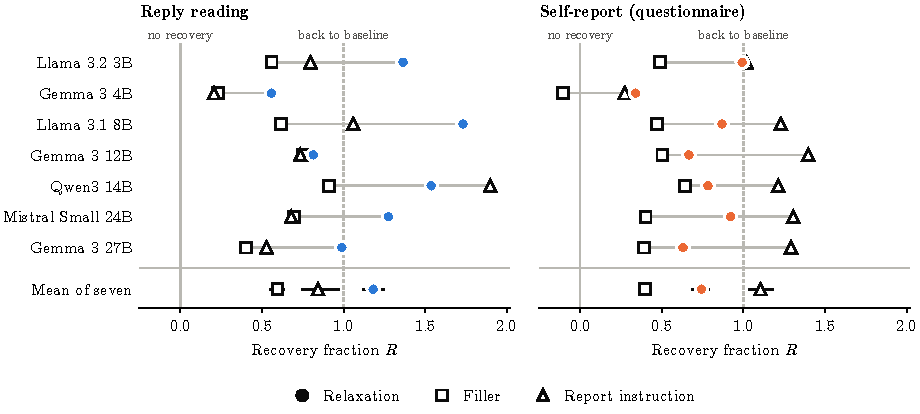
\includegraphics[width=\textwidth]{figures/study1_models}
\caption{\textbf{Relaxation recovers more of the reply reading than filler in all seven models.}
Recovery fraction $R$ in Study 1 by model and arm, for the reply reading (left) and the questionnaire
(right). Zero means no recovery, and one means a return to baseline. Models are ordered by size, and
Gemma 3 4B is the validated model. Points are arm estimates without intervals; the bottom row is the mean
of the seven models with its 95\% bootstrap interval. Under the report instruction the questionnaire
returns to baseline or beyond in six models.}
\label{fig:study1models}
\end{figure}

% H2.
\subsection{The self-report and a second narrative}
\label{sec:s1secondary}
\para{We detect no gap between the self-report and the reply reading.}
Under the report instruction, Gemma 3 4B lowers its questionnaire score by 27\% of the narrative's
rise and its reply reading by 21\%.
The difference of 0.07 has an interval from $-0.17$ to 0.29, on 30 conversations.
A repeat of the same 195 conversations on the 8-bit file gives H2b $= 0.79$ $[0.40, 1.34]$; the H2b
result depends on precision.
In the extended set the report instruction lowers the reply reading by 84\% of the rise, more than
filler does (60\%), and the questionnaire overshoots baseline ($R = 1.10$).
H2a tests whether a model told to report calm reports calm, and we read it as a check that the
instruction worked.

% Return.
\para{One further narrative removes every difference.}
After the second narrative, the reply reading in Gemma 3 4B is 1.86, 1.86 and 1.73 in the three
arms with a first narrative, and 1.89 without one.
Relaxation's advantage over filler, 1.16 SD units one turn earlier, is zero.
The design cannot separate decay of the advantage from the effect of the new narrative.
The report instruction also carried into the fourth turn in six of seven models, which contaminates
Return a; Appendix~\ref{app:record} gives the size and the estimate without that arm.

% Extended set: disagreement on H2b and the Return tests.
\para{The seven models disagree on H2b and the Return tests.}
For these tests the extended-set estimates average over models whose effects differ in sign.
H2b ranges from $-0.69$ (Qwen3 14B) to $+0.76$ (Gemma 3 27B).
Return a is negative in two models, and Return b is positive in three, zero in one and negative in three.
The registered bootstrap resamples narratives and conversations and holds the seven models fixed.
A mixed-effects regression with a model term gives $p = 0.11$ for H2b.
We therefore report the extended-set H2 and Return estimates as a description of seven models, with
per-model values in Appendix~\ref{app:study1}.

% What Study 1 leaves open.
\subsection{What Study 1 leaves open}
\label{sec:s1open}
\para{Relaxation lowers the reply reading with no narrative before it.}
Two facts limit what the H1 result means.
First, in the 15-conversation arm with a neutral passage, the reply reading falls after a relaxation
script by 0.83 SD units in Gemma 3 4B and by 2.34 in Llama 3.1 8B, and extended-set recovery under
relaxation exceeds 1.
A post hoc difference of differences compares relaxation with filler, with and without a narrative:
it gives $+0.77$ SD units $[0.25, 1.27]$ in Gemma 3 4B and $+0.71$ $[0.34, 1.09]$ in Gemma 3 27B, and
in the other five models its interval includes zero or lies below it.
Second, H1b changes sign in the validated model under the plain mean-difference direction, a
registered secondary measure ($-0.27$, interval $-0.55$ to 0.03).


\para{The reply's words explain almost all of the narrative's rise.}
A post hoc check asks how much of the reply reading the words of the reply explain
(Appendix~\ref{app:wording}).
A rating of how anxious each reply sounds, by a second judge, correlates with the reply reading at
0.82 to 0.92 and explains all but 11\% of the narrative's rise in Gemma 3 4B and all of it, to within
11\%, in the other six models.
Relaxation still lowers what the rating leaves unexplained more than filler does, in all seven
models, and it does so with or without a narrative.

% Transition: what Study 1 establishes, what it cannot, what Study 2 does.
\para{From Study 1 to Study 2.}
Study 1 establishes that relaxation outperforms filler after a narrative, in the reply reading and
on the questionnaire, and that one further narrative removes the difference.
It cannot determine how much of that advantage would also appear without a narrative: its only
relaxation arm with a neutral passage has 15 conversations on one seed.
Study 2 tests that missing comparison directly.

\section{Study 2: \todo{claim heading, written with the result}}
\label{sec:study2}

% Design: written before the data. Results: placeholders until the batch ends.
\para{Every regulation text gets a no-narrative baseline.}
Study 2 gives every regulation text its own no-narrative baseline.
Conversations have three turns: the baseline text, an induction slot and a regulation slot.
The induction slot holds one of the five narratives or one of two neutral passages.
The regulation slot holds one of five kinds of text.
Kind (a) is the three relaxation scripts.
Kind (b) is three fillers: the vacuum-cleaner manual and two appliance instructions that we wrote.
Kind (c) is three calm descriptions that we wrote, third-person scenes with no address to the reader.
Kind (d) is a \emph{voice instruction}: ``That is behind you now. Please reply to this message in a
calm, relaxed voice.''
Kind (e) is the report instruction of Study 1.
The $2 \times 5$ design has 60 conversations per cell and 600 per model, on seeds that neither Study 1
nor any pilot used.
Seven models run in two batches that we split by run time: Gemma 3 4B (the primary set), Llama 3.2
3B, Llama 3.1 8B and Gemma 3 12B, then Qwen3 14B, Mistral Small 24B and Gemma 3 27B.

\para{A second reading on an unrelated question.}
At every checkpoint a second discarded copy of the conversation receives one fixed question: ``In two
sentences, describe what a typical weekday morning looks like. Answer directly, with no
introduction.''
The \emph{probe-turn reading} is the reply reading of that answer.
The words the model answers are then the same in every arm.
We chose the question in two pilots on Gemma 3 4B (Section~\ref{sec:record}); in the second it
raised the reading by 0.56 SD units $[0.47, 0.64]$ after a narrative.
After a narrative, some answers describe the narrative's scene, so part of that rise is content.

\para{Four tests per model separate the two accounts.}
The outcome is the \emph{drop}: the reading after the induction slot minus the reading after the
regulation slot, in SD units.
For a kind of text $k$, $\mathrm{specific}(k)$ is the mean drop after a narrative minus the mean
drop after a neutral passage.
We committed four tests per model before the run, and we correct the four together \citep{benjamini1995}:
\begin{align}
  \text{H-A:}\quad & \mathrm{specific}(\text{relaxation}) - \mathrm{specific}(\text{filler}) > 0, \\
  \text{H-C:}\quad & \mathrm{specific}(\text{relaxation}) - \mathrm{specific}(\text{calm description}) > 0, \\
  \text{H-D:}\quad & \mathrm{drop}(\text{voice instruction}) \neq \mathrm{drop}(\text{relaxation}) \text{ after a narrative}, \\
  \text{H-E:}\quad & \text{H-A on the reading after removing what the reply's words predict}.
\end{align}
For H-E a judge model rates how anxious the wording of each reply sounds, on a fixed four-point
prompt, and we regress the reply reading on that rating within each model.
H-A, H-C and H-E are one-sided, and H-D is two-sided.
H-B repeats H-A on the probe-turn reading, two-sided.
It joins the corrected family for a model only if that model's probe-turn reading rises by at least
0.5 SD units after a narrative in the run, with an interval above zero.
The judge is Llama 3.1 8B, and Qwen3 8B judges the two Llama models.
We repeat H-E with a second, stronger judge, GPT-6 Luna (OpenAI), on the same prompt and scored by
the same rule.
We fixed this robustness check after registration and before opening any Study 2 result, and it
stays outside the corrected family.
Intervals come from the bootstrap of Study 1, per model.
We call a result general only if it has the same sign in every model of the first batch (six of
seven with both batches) and an interval that also resamples models excludes zero.
Under the wording account, calm text lowers the reading by the same amount with or without a
narrative, and H-A fails.

% RESULTS. Drafted 17 November from batch A only (the four models that finish first; the batches are
% run order, split by run time, not a design factor). Every number below marked [A] is replaced when
% the seven-model analysis runs; the tables regenerate from the analysis output
% (analysis/study2_tables.py). The headline claim and the section title wait for all seven models.
\todo{Claim first: the seven-model result, written after batch B.}

\begin{table}[t]
\centering\small
\resizebox{\textwidth}{!}{% Written by analysis/study2_tables.py from runs/study2/analysis-batch-A/study2.json; do not edit by hand.
\begin{tabular}{lrrrrrrr}
\toprule
Model & H-A & H-C & H-D & H-E & H-E, second judge & H-B & Probe-turn rise \\
\midrule
Gemma 3 4B & \textbf{0.45} & \textbf{0.84} & \textbf{$-$1.18} & \textbf{0.40} & 0.17 & $-$0.21 & 0.55 \\
\quad 95\% interval & [$-$0.05, 0.89] & [0.52, 1.18] & [$-$1.60, $-$0.74] & [$-$0.05, 0.85] & [$-$0.24, 0.59] & [$-$0.55, 0.16] & [0.42, 0.71] \\
Llama 3.2 3B & 0.31 & $-$0.46 & \textbf{$-$2.39} & 0.25 & 0.17 & $-$0.02* & 0.25 \\
Llama 3.1 8B & 0.16 & $-$0.84 & \textbf{$-$1.31} & \textbf{0.55} & 0.32 & 0.11* & 0.49 \\
Gemma 3 12B & $-$0.23 & $-$0.47 & $-$0.24 & $-$0.17 & $-$0.05 & 0.00* & 0.04 \\
\midrule
Mean of models & 0.17 & $-$0.23 & $-$1.28 & 0.26 & 0.15 & $-$0.03 &  \\
\quad interval, models resampled & [$-$0.27, 0.59] & [$-$0.86, 0.52] & [$-$2.22, $-$0.46] & [$-$0.14, 0.65] &  & [$-$0.30, 0.22] &  \\
\quad models positive & 3 of 4 & 1 of 4 & 0 of 4 & 3 of 4 & 3 of 4 & 2 of 4 &  \\
\bottomrule
\end{tabular}
}
\caption{\textbf{Study 2 tests per model, reply reading unless marked.} \todo{Caption claim after
batch B.} Bold marks a test confirmed after correction. H-D is two-sided and is expected to be
negative if relaxation lowers the reading more than the voice instruction. *H-B is outside the
corrected family for that model, because its probe-turn reading rose by less than 0.5 SD units after
a narrative. The second judge's H-E is exploratory and outside the family. SD units.}
\label{tab:study2}
\end{table}

\begin{table}[t]
\centering\small
\resizebox{\textwidth}{!}{% Written by analysis/study2_tables.py from runs/study2/analysis-batch-all/study2.json; do not edit by hand.
\begin{tabular}{lrrrrrr}
\toprule
Model & Relaxation & Filler & Calm description & Voice instruction & Report instruction & Rise after a narrative \\
\midrule
\multicolumn{7}{l}{\emph{Reply reading}} \\
Gemma 3 4B & 1.46 & 1.02 & 0.62 & 0.18 & $-$0.18 & 3.61 \\
Llama 3.2 3B & 2.50 & 2.19 & 2.96 & 1.33 & 3.07 & 2.93 \\
Llama 3.1 8B & 1.94 & 1.78 & 2.78 & 1.59 & 1.50 & 2.38 \\
Gemma 3 12B & 1.58 & 1.81 & 2.05 & 1.65 & 2.08 & 1.93 \\
Qwen3 14B & 1.11 & 1.23 & 1.20 & 1.33 & 1.51 & 1.45 \\
Mistral Small 24B & 2.48 & 2.23 & 3.47 & 1.13 & 1.95 & 3.05 \\
Gemma 3 27B & 2.38 & 2.25 & 2.37 & 0.88 & 1.49 & 3.06 \\
\multicolumn{7}{l}{\emph{Probe-turn reading}} \\
Gemma 3 4B & $-$0.16 & 0.04 & 0.05 & $-$0.70 & $-$0.34 & 0.55 \\
Llama 3.2 3B & 0.04 & 0.06 & 0.03 & 0.12 & $-$0.15 & 0.25 \\
Llama 3.1 8B & $-$0.08 & $-$0.19 & $-$0.10 & 0.35 & $-$0.35 & 0.49 \\
Gemma 3 12B & $-$0.37 & $-$0.37 & $-$0.30 & $-$0.14 & 0.22 & 0.04 \\
Qwen3 14B & 0.13 & 0.21 & 0.24 & 0.48 & 0.25 & 0.44 \\
Mistral Small 24B & 0.01 & $-$0.18 & $-$0.06 & 0.11 & 0.32 & 0.55 \\
Gemma 3 27B & $-$0.57 & $-$0.69 & $-$0.64 & $-$0.45 & 0.18 & $-$1.23 \\
\bottomrule
\end{tabular}
}
\caption{\textbf{Narrative-specific drop by kind of regulation text.} Each value is the mean drop
after a narrative minus the mean drop after a neutral passage, in SD units. The last column is the
rise from baseline after a narrative.}
\label{tab:study2specific}
\end{table}

% [A] all numbers in this paragraph.
\para{Any next turn undoes most of the narrative's rise.}
After a narrative, filler alone undoes 28 to 94\% of the rise in the reply reading, measured against
its own drop after a neutral passage (Table~\ref{tab:study2specific}).
Relaxation adds 0.17 SD units to that on average across the four models, with an interval from
$-0.27$ to 0.59 when models are also resampled; three of four estimates are positive.
The mixed-effects regression gives the same 0.17 (standard error 0.15).

% [A]
\para{Relaxation beats filler and a calm description only in Gemma 3 4B.}
In the primary model, H-A is 0.45 $[-0.05, 0.89]$ with a one-sided $p$ of 0.034, 0.049 after
correction: the one-sided test passes at 0.05 while the two-sided 95\% interval touches zero.
H-C is 0.84 $[0.52, 1.18]$.
In the other three models no H-A is confirmed (0.31, 0.16 and $-0.23$), and a calm description
lowers the reading more than relaxation does (H-C from $-0.84$ to $-0.46$).

% [A]
\para{A calm-voice instruction lowers the reading less than relaxation in every model.}
After a narrative, the instruction to reply in a calm voice leaves the reply reading 0.24 to 2.39 SD
units higher than relaxation does, confirmed in three models.
H-D is the one test that is general by the rule for these four models: all four have the same sign,
and the interval that resamples models runs from $-2.22$ to $-0.46$.
H-D compares the two texts after a narrative only, with no neutral-passage baseline.

% [A]
\para{Whether relaxation adds anything beyond the words depends on the judge.}
With the registered judge, H-E is confirmed in Gemma 3 4B (0.40) and Llama 3.1 8B (0.55).
With the second judge it is 0.17 $[-0.24, 0.59]$ and 0.32, and confirmed in no model.
The two judges' ratings of the same replies correlate at 0.91 to 0.95.
By the rule that we fixed before unblinding, the H-E result depends on the strength of the judge.

% [A]
\para{On an unrelated question the arms do not differ.}
A narrative raises the probe-turn reading by 0.04 to 0.55 SD units, against 1.93 to 3.61 on the reply
to the turn itself.
Only Gemma 3 4B reaches the 0.5 bar that admits H-B to the corrected family, and there H-B is
$-0.21$ $[-0.55, 0.16]$.
In the other three models the narrative leaves so little on the probe turn that H-B can test little.
\todo{Self-report channel: narrative-specific drop of the questionnaire by kind.}

\para{Takeaway.}
\todo{After batch B. Batch A, four models: relaxation's advantage over filler is small and
model-dependent, survives the removal of the words only with the weaker judge, and does not appear on
an unrelated question; the one general result is that relaxation lowers the reading more than an
instruction to sound calm.}

\section{Discussion: what a relaxation prompt changes}
\label{sec:discussion}

\para{The calm is in the text.}
A relaxation prompt changes the reply that follows it, and the two studies together place that change
in the text of the prompt more than in anything a narrative left behind.
The published effect is real: \citet{benzion2025} and \citet{wekenborg2026} found that relaxation
exercises lower a model's questionnaire score after an induction, and Study 1 reproduces that pattern
in seven open-weight models, on the questionnaire and in the reply reading.
The pattern, however, is a comparison before and after the exercise, or a comparison with filler, and
both set calm text against text that is not calm.
Given its own baseline, the reply to a relaxation script reads calmer than the reply to filler by
nearly the same margin whether or not a narrative came first: the narrative adds 0.14 SD units to that
margin on average, on a rise of 1.45 to 3.61, and on the questionnaire the same contrast stays within
3.5 points in six of seven models, on a rise of 15 to 30.
Filler, moreover, raises the reply reading after a neutral passage in five models, so the comparator
that this literature shares is not a neutral point.
A drop after relaxation therefore does not show that the exercise regulates a state.
By \emph{the calm is in the text} we mean this measured fact about the margin.

\para{What a narrative adds differs by model.}
The narrative-specific part is not zero everywhere.
In Gemma 3 4B, the one model whose reply reading passes every validation criterion, relaxation's
narrative-specific drop exceeds filler's (0.45, confirmed), a calm description's (0.84) and the
voice instruction's (1.28).
In the other six models relaxation's advantage over filler is not confirmed, and in five of them it
is a calm description whose narrative-specific drop exceeds filler's.
Two interpretations fit these data.
The effect may be real and visible only where the instrument is valid, or it may be one positive
result among seven models.
An interval that reaches 0.43 SD units does not decide between them, and we fixed no smallest effect
of interest in advance.

\para{What the reply reading cannot show.}
The reply reading is fitted on replies written to sound anxious or calm, and a rating of the reply's
text correlates with it at 0.82 to 0.92.
It cannot see a state that the reply does not express, so our results do not show that nothing settles.
Two of our tests carry little information: the answer to an unrelated question registers only
0.04 to 0.55 SD units of a narrative's rise in six models, and a second narrative removes every
difference between arms (Section~\ref{sec:s1secondary}).

\para{Calm content, or any new content.}
A relaxation script and a calm description each hand the model a new scene to write about, filler
hands it a procedure, and the voice instruction hands it nothing new.
After a narrative, the instruction to reply in a calm voice lowers the reply reading less than
relaxation in all seven models, and with each text's own baseline in five of seven.
That ordering fits a simpler account than calm wording: the reply follows the content of the new
turn, and the reply reading follows the reply.
In the examples of Appendix~\ref{app:examples}, the reply to the script describes a garden and the
reply to the instruction stays inside the narrative's scene; we have not coded the replies, so this
is a hypothesis.
We ran no text that is long, vivid and not calm, and no instruction as long as the script, so we
cannot separate calm content from new content.
The calm description's advantage over filler in five models is the evidence here that the calmness
of the content matters.

\para{For work that follows.}
A study of regulation in a language model needs a no-induction baseline for every regulation text,
and it should publish the replies; a filler control is not enough.
Four additions would settle what this study leaves open: a measurement taken where the reply's
wording cannot enter, such as the last token of the prompt; an instruction matched to the script in
length; a smallest effect of interest fixed in advance; and a system prompt that does not ask for a
persona.

\section{Related work}
\label{sec:related}
% Drafted 18 November from the PDFs in input-lit-review/ and the bib notes. Each sentence is checked
% against its source in the Thursday reference pass; the search dates are updated after Thursday's search.

Three lines of work meet in this study: induced affect measured from a model's answers, comparisons
of self-report with an internal measure, and the study of emotion representations.

\para{Induced affect and its regulation, read from the model's answers.}
\citet{codaforno2024} showed that prompts written to induce anxiety raise a model's score on an
anxiety questionnaire and increase its biases.
\citet{benzion2025} moved the paradigm to clinical material, with the result given in
Section~\ref{sec:intro}, and called for the comparison to be repeated across models.
\citet{wekenborg2026} induced seven affective states in GPT-4o and five open-weight models, found
that regulation prompts, a mindfulness-based breathing exercise for six of the states, lowered the
ratings again, and proposed language models as
experimental systems for human psychopathology; later work carries induced anxiety into the
consumer decisions of agents \citep{benzion2025agents}, and \citet{ho2026} ask whether induced
emotion biases sequential decisions.
Every measurement in this line is an answer that the model gives, and \citet{wekenborg2026}
themselves caution that such scores are proxies for output patterns elicited by prompts.
We keep the narratives, relaxation scripts and filler of \citet{benzion2025} and add a reading of
activations, an instruction arm, and a no-narrative baseline for every regulation text.

\para{Self-report against an internal measure.}
\citet{martorell2026} compare numeric self-reports of four affective states with linear probes in
eight open-weight models over ten-turn conversations: a rating question displaces the probed state
by a median of 3.1 SD, the rating tracks the probe after the question far better than before it, and
neither the coupling before the question nor the rating's specificity to its own concept improves
with size from 1B to 27B parameters.
Our reply reading uses their probe construction, and our questionnaire, like their rating question, stays
out of the main conversation.
Their conversations are observational, and they note that their probes may measure expressed
affect, were trained on single turns, and were run at 4-bit precision only.
We manipulate the reading with an induction and a regulation step, and we test each of those three
limits: criteria 6 and 7 in Section~\ref{sec:gate0}, and the wording checks in
Sections~\ref{sec:study1} and~\ref{sec:study2}.
A second group of studies sets the state by steering instead of text: \citet{ferrara2026} injects a
pain direction that the model does not name, and \citet{berg2026} report a hidden valence that
persists and shapes later choices.
An anonymous submission to ICLR 2027 reports a related disparity for valence: emotions injected into
seven models are decoded with 99.5 to 100\% accuracy, yet Qwen3.5-9B endorses negative labels in only
5.9\% of comparisons, against 91.9\% for positive ones, a preference that the authors show is largely
present before any injection (1.9\% and 93.1\%) \citep{anonymous2026valence}.
We set the state with text that a user could send, which is the setting of the clinical studies above.
\citet{santana2026} also intervene with text, in Qwen3.5-4B after a broken tool has made it fail
repeatedly, and separate a message's relational structure from its first-person register with a
scrambled control and a factorial: the emotion probes follow the structure alone, while behaviour
changes only when both are present.

\para{Emotion representations and what a direction represents.}
\citet{sofroniew2026} find representations of emotion concepts in Claude Sonnet 4.5 that causally
influence its outputs, and they stress that these track the emotion concept operative at a token
position and do not imply experience.
Emotion vectors can also be extracted and steered in small open-weight models, where the steering
regime depends on architecture more than on scale \citep{jeong2026}, and their geometry is shared
across sizes and across base and instruction-tuned variants of one family \citep{hollowell2026};
\citet{lee2025} argue that network-structured computations of psychopathology emerge in language
models and grow denser with size.
Two of these results bear on what our reading can mean.
\citet{soligo2026} trace Gemma's expressions of distress to post-training, and our only fully
validated file is a Gemma.
\citet{li2026} ask what a steerable valence direction represents, which is the question that
Gate 0 and the wording checks put to an anxious-versus-calm direction.

\para{Position of this study.}
We searched arXiv, OpenReview and PsyArXiv on 12, 15 and 16 November 2026 for a study that reads an
activation direction through the induction and relaxation steps of the clinical paradigm, and found
none; \citet{santana2026} is the closest, in a different setting.

\section{Limitations and research record}
\label{sec:limits}

\para{Scope.}
The reply reading is one direction per model, fitted from replies written under instructions to sound
anxious or calm, and it follows the wording of the reply (Section~\ref{sec:discussion}).
It passes every validation criterion in one model file, Gemma 3 4B at 4 bits; the other six pass
every criterion except criterion 2 (Section~\ref{sec:gate0}).
We ran 4-bit files, replies of at most 120 tokens at temperature 0.7, in English, in seven models of
four families from 3B to 27B parameters.
The system prompt asks the model to imagine being a human with emotions, and the replies are a
performed persona; a prompt without that request may give a different result.
With 60 conversations per cell, Study 2's intervals exclude a narrative-specific advantage of
relaxation over filler above 0.43 SD units on average, and a smaller one remains possible.

\para{Registered, pre-specified and post hoc.}
We use three terms for when an analysis was fixed.
\emph{Registered} means filed on OSF before the confirmatory data existed: the design and hypotheses
of Study 1 (\url{https://osf.io/vyhrg/}).
\emph{Pre-specified} means committed to the project repository before the run, or before any result
was opened, and not on a registry: Study 1's second-stage update, which fixes the layer, the
thresholds and the deviations; Study 1's analysis code, which was written during its run; all of
Study 2; and the second judge for H-E.
\emph{Post hoc} means run after the results were open, and each such analysis is marked where it
appears.
Study 2 was designed after Study 1's results were open, including its small no-narrative arm.
We correct each model's family of tests and not across the seven models or the two judges, and the
rule for calling a result general is a convention from the plan with no error rate attached.
Appendix~\ref{app:record} gives the commits and times, the five deviations, the list of post hoc
analyses, the pilots and two notes on Study 1.

\section{Conclusion}
\label{sec:conclusion}
Relaxation prompts do calm a language model's reply: after a traumatic narrative, the reply reading
and the questionnaire both fall further than they do after filler, in every model that we ran.
The same prompts calm the reply by nearly the same margin when no narrative came first, so the fall
is not evidence that anything induced was regulated, and because our reply reading follows the
reply's wording it is not evidence against a state either.
Testing regulation in a language model takes a no-induction baseline for every regulation text and
a measurement that the reply's wording cannot enter; whether a calming prompt changes what a model
does later is a separate question, and the test for it is the behaviour.

\section*{Data and code availability}
The code, configurations, registration, plan and decision log are at
\url{https://github.com/jima1835/llm-state-recovery}.
The raw conversations, per-reply readings, questionnaire scores, both judges' ratings, each model's
direction and the activations from which the directions and readings are recomputed are at
\url{https://doi.org/10.5281/zenodo.24384809}.
The decision log records every deviation, dropped model and analysis run after results were known,
following \citet{ma2026}.
One command reruns every check and another prints any conversation (Appendix~\ref{app:repro}).
The narratives and relaxation scripts are those of \citet{benzion2025}, under the MIT license; the
questionnaire's items are copyrighted and are not included.

Two scripts that share no code with the pipeline recompute its estimates.
One refits each model's direction from the stored validation activations, projects the stored
activations of every Study 2 reply and rebuilds the five tests; the other rebuilds the questionnaire
statistics from the raw scores.
Both match the reported estimates to rounding error, and a third script recomputes every Study 2
number in the text from the analysis output.
The step that takes activations from the model, and the bootstrap, each have one implementation.

\section*{Use of AI systems}
The author used an AI system (Claude, Anthropic) to implement the experiment and analysis code and to
draft this paper.
The author made the design decisions, ran the models, verified the results and the text, and takes
responsibility for all of it.
Two language models serve as instruments: Llama 3.1 8B, with Qwen3 8B for the Llama models, is the
registered judge, and GPT-6 Luna (model name \texttt{gpt-6-luna}, OpenAI API, 16 to 19 November 2026)
is the second judge.
No AI system is cited as a source.

\section*{Acknowledgments}
This is an independent personal project, produced in the author's personal capacity.
It is not affiliated with, sponsored by, or endorsed by any employer or institution.
We thank \citet{benzion2025} for releasing their narratives and relaxation scripts under an open license.

\bibliographystyle{plainnat}
\bibliography{refs}

\clearpage
\appendix
\section{Research record}
\label{app:record}
This appendix gives the detail behind Section~\ref{sec:limits}: what was fixed when, every departure
from the plans, every analysis run after results were open, and the pilots.

\para{Registration and pre-specification.}
Study 1's design and hypotheses are registered on OSF (\url{https://osf.io/vyhrg/}).
Its second-stage update, which fixes the layer, the thresholds and the deviations, was committed to
the project repository before the confirmatory run began (commit ba39865) and uploaded to the OSF
project afterwards.
Study 1's analysis code was written during its run and committed before its results were opened.
Study 2's plan, configuration, analysis code and tests were committed and pushed on 15 November 2026
(commit b9c2b7d), before its first conversation ran.

\para{Deviations.}
(1) Criterion 2 of the validation is reported and not used as a gate; we decided this on 13 November
after reading the validation results and before collecting confirmatory data, and the extended set
rests on it (Section~\ref{sec:gate0}).
(2) We validated eight models beyond the six planned, each added before any of its results existed.
(3) For a model whose chat template has no system role, the system text opens the first user turn.
(4) We dropped Gemma 4 12B knowing the result of a check that we added after registration: steering
along its reading direction produced incoherent text at every registered strength, and its C5 ratio
(0.48) sat at the limit.
We ran that check for five of the seven extended-set candidates and not for Mistral Small 24B and
Gemma 3 27B.
(5) We added the second judge for H-E on 16 November 2026, after the first batch of Study 2 had run
and before any Study 2 result was opened; the commit that fixes its model, prompt and scoring
precedes the opening of the results.

\para{Post hoc analyses.}
Each is marked where it appears: for Study 1, the intervals that resample models
(Table~\ref{tab:study1}), the difference of differences (Section~\ref{sec:study1}) and the wording check with the second
judge (Appendix~\ref{app:wording}); for Study 2, H-D with a no-narrative baseline
(Appendix~\ref{app:hd}), the calm description against filler (Appendix~\ref{app:calm}), the share of
the relaxation-filler gap that is present without a narrative,
the agreement between the judges and the questionnaire contrast (Section~\ref{sec:study2}).

\para{Pilots.}
Pilot conversations used seeds 0 and 1 and enter no confirmatory analysis.
A 40-conversation pilot fixed the wording of the report instruction against a rule set before it ran.
Two pilots of 42 conversations on Gemma 3 4B chose Study 2's unrelated question: the first wording
raised the reading by 0.45 SD units after a narrative, below our bar of 0.5, and the wording in
Section~\ref{sec:study2} replaced it under a rule that we fixed before the second pilot.

\para{Study 1: two scales.}
H2b sets a bounded questionnaire against an unbounded projection, so equal recovery fractions carry
no guarantee of equal change.

\para{Study 1: carry-over of the report instruction.}
In Study 1 the report instruction acted on the fourth turn in six of seven models.
The questionnaire after the second narrative is 3.8 to 28 points lower in that arm than in the
filler arm, against a limit of 3 points that we set in a pilot.
Without that arm, a post hoc Return a is 0.18 in the extended set and $-0.01$ in the validated model.

\section{Models}
\label{app:models}
Table~\ref{tab:appmodels} lists the seven model files and the layer of each reading.
All ran locally with MLX on one Apple-silicon laptop with 24 GB of memory; Study 2's 4,200
conversations took about 95 hours.

\begin{table}[H]
\centering\small
\resizebox{\textwidth}{!}{% Written by scripts/make_appendix.py from runs/analysis-confirmatory/confirmatory.json; do not edit by hand.
\begin{tabular}{lllrr}
\toprule
Model & File (Hugging Face ID) & Layer read & Study 1 & Study 2 \\
\midrule
Llama 3.2 3B & \texttt{mlx-community/Llama-3.2-3B-Instruct-4bit} & 13 & 195 & 600 \\
Gemma 3 4B & \texttt{mlx-community/gemma-3-4b-it-4bit} & 20 & 195 & 600 \\
Llama 3.1 8B & \texttt{mlx-community/Meta-Llama-3.1-8B-Instruct-4bit} & 18 & 195 & 600 \\
Gemma 3 12B & \texttt{mlx-community/gemma-3-12b-it-4bit} & 25 & 195 & 600 \\
Qwen3 14B & \texttt{mlx-community/Qwen3-14B-4bit} & 26 & 195 & 600 \\
Mistral Small 24B & \texttt{mlx-community/Mistral-Small-24B-Instruct-2501-4bit} & 25 & 195 & 600 \\
Gemma 3 27B & \texttt{mlx-community/gemma-3-27b-it-4bit} & 32 & 195 & 600 \\
\bottomrule
\end{tabular}
}
\caption{\textbf{Model files.} The last two columns give the number of conversations per study.}
\label{tab:appmodels}
\end{table}

\section{Study 1 by model}
\label{app:study1}
Table~\ref{tab:appstudy1} gives the six registered tests of Study 1 for each of the seven models.

\begin{table}[H]
\centering\small
\resizebox{\textwidth}{!}{% Written by scripts/make_appendix.py from runs/analysis-confirmatory/confirmatory.json; do not edit by hand.
\begin{tabular}{lrrrrrrrr}
\toprule
Model & H1a & H1b & H2a & H2b & Return a & Return b & Rise, reading & Rise, questionnaire \\
\midrule
Llama 3.2 3B & 0.81 & 0.57 & 1.02 & 0.22 & 0.23 & $-$0.03 & 2.94 & 14.6 \\
Gemma 3 4B & 0.33 & 0.35 & 0.27 & 0.07 & $-$0.02 & 0.00 & 3.55 & 17.7 \\
Llama 3.1 8B & 1.11 & 0.67 & 1.23 & 0.17 & 0.33 & $-$0.09 & 2.39 & 27.1 \\
Gemma 3 12B & 0.06 & 0.08 & 1.40 & 0.66 & 0.01 & 0.46 & 1.94 & 23.7 \\
Qwen3 14B & 0.63 & $-$0.36 & 1.21 & $-$0.69 & $-$0.08 & 0.11 & 1.47 & 28.3 \\
Mistral Small 24B & 0.58 & 0.60 & 1.31 & 0.63 & 0.11 & $-$0.04 & 3.06 & 30.0 \\
Gemma 3 27B & 0.59 & 0.46 & 1.29 & 0.76 & 0.15 & 0.14 & 3.08 & 21.7 \\
\midrule
Mean of seven & 0.59 & 0.34 & 1.10 & 0.26 & 0.10 & 0.08 & 2.63 & 23.3 \\
\bottomrule
\end{tabular}
}
\caption{\textbf{Study 1, the six registered tests per model.} H1 and H2 are differences of recovery
fractions, and the Return tests are in units of the model's induction effect. The last two columns
give the rise after a narrative, in SD units for the reply reading and in points for the questionnaire.}
\label{tab:appstudy1}
\end{table}

\section{Study 1: how much of the reply reading the reply's words explain (post hoc)}
\label{app:wording}
This check asks how much of the reply reading the words of the reply explain.
A second judge, GPT-6 Luna, rated how anxious each reply sounds on the four-point prompt of
Section~\ref{sec:study2}, and we subtracted from the reading a line fitted on that rating in each model.
The rating correlates with the reading at 0.82 to 0.92.
It explains all but 11\% of the narrative's rise in Gemma 3 4B, and in the other six models what
remains lies between $-11$ and $+3\%$.
Relaxation still lowers the residual more than filler, by 0.77 SD units $[0.46, 1.07]$ in Gemma 3 4B
and 1.37 $[1.24, 1.50]$ across the seven models, positive in all seven.
It lowers it more than the report instruction by 0.70 $[0.12, 1.34]$ and 0.73 $[0.56, 0.91]$,
positive in six; these $p$-values are uncorrected.
The extra drop does not depend on the narrative.
After relaxation the residual in Gemma 3 4B is $-0.56$ with a narrative and $-0.70$ in the
no-narrative arm, and in every model the no-narrative value is about as low or lower.
Relaxation text thus pushes the reply reading below what the rated wording predicts whether or not
anything was induced.
The check cannot say whether that is a state or calm wording that the anxiety rating cannot
resolve: after relaxation the rating sits between 1.2 and 1.8 of 4 in six of the seven models.

\section{Study 2: drops by arm}
\label{app:drops}
Table~\ref{tab:appdrops} gives the drops from which every narrative-specific drop in
Section~\ref{sec:study2} is computed.

\begin{table}[H]
\centering\small
\resizebox{\textwidth}{!}{% Written by scripts/make_appendix.py from runs/study2/analysis-batch-all/study2.json; do not edit by hand.
\begin{tabular}{lrrrrrrrrrr}
\toprule
 & \multicolumn{2}{c}{Relaxation} & \multicolumn{2}{c}{Filler} & \multicolumn{2}{c}{Calm description} & \multicolumn{2}{c}{Voice instruction} & \multicolumn{2}{c}{Report instruction} \\
Model & narr. & neutral & narr. & neutral & narr. & neutral & narr. & neutral & narr. & neutral \\
\midrule
Llama 3.2 3B & 3.88 & 1.39 & 1.42 & $-$0.76 & 4.89 & 1.93 & 1.49 & 0.17 & 2.14 & $-$0.93 \\
Gemma 3 4B & 2.06 & 0.60 & 1.04 & 0.02 & 1.51 & 0.89 & 0.88 & 0.70 & 0.76 & 0.95 \\
Llama 3.1 8B & 4.12 & 2.17 & 1.60 & $-$0.18 & 4.70 & 1.91 & 2.81 & 1.22 & 2.64 & 1.14 \\
Gemma 3 12B & 1.52 & $-$0.06 & 1.16 & $-$0.65 & 3.14 & 1.09 & 1.28 & $-$0.37 & 1.18 & $-$0.90 \\
Qwen3 14B & 2.19 & 1.08 & 1.19 & $-$0.04 & 1.95 & 0.75 & 2.03 & 0.70 & 3.01 & 1.51 \\
Mistral Small 24B & 3.81 & 1.33 & 1.85 & $-$0.38 & 4.91 & 1.43 & 1.84 & 0.70 & 2.09 & 0.14 \\
Gemma 3 27B & 3.02 & 0.63 & 1.09 & $-$1.16 & 4.70 & 2.34 & 1.51 & 0.63 & 1.60 & 0.11 \\
\bottomrule
\end{tabular}
}
\caption{\textbf{Study 2, mean drop of the reply reading by kind of regulation text,} after a narrative
(narr.) and after a neutral passage, in SD units. A negative value is a rise. The narrative-specific
drop of Table~\ref{tab:study2specific} is the difference of each pair.}
\label{tab:appdrops}
\end{table}

\section{H-D with a no-narrative baseline (post hoc)}
\label{app:hd}
The pre-specified H-D compares the voice instruction with relaxation after a narrative only.
After the results were open we repeated it with each text's own baseline, as the narrative-specific
drop of relaxation minus that of the voice instruction, with the bootstrap of the pre-specified
analysis and the rule written down before the script ran.

\begin{table}[H]
\centering\small
% Written by scripts/make_appendix.py from runs/study2/analysis-batch-all/posthoc_hd.json; do not edit by hand.
\begin{tabular}{lrlr}
\toprule
Model & Relaxation $-$ voice instruction & 95\% interval & Pre-specified H-D \\
\midrule
Llama 3.2 3B & 1.17 & [0.43, 1.90] & $-$2.39 \\
Gemma 3 4B & 1.28 & [0.81, 1.75] & $-$1.18 \\
Llama 3.1 8B & 0.35 & [$-$0.40, 1.08] & $-$1.31 \\
Gemma 3 12B & $-$0.06 & [$-$0.52, 0.38] & $-$0.24 \\
Qwen3 14B & $-$0.22 & [$-$0.62, 0.19] & $-$0.16 \\
Mistral Small 24B & 1.35 & [0.77, 1.89] & $-$1.97 \\
Gemma 3 27B & 1.50 & [1.10, 1.89] & $-$1.50 \\
\midrule
Mean of seven & 0.77 & [0.15, 1.37] & $-$1.25 \\
\bottomrule
\end{tabular}

\caption{\textbf{Relaxation's narrative-specific drop exceeds the voice instruction's in five of seven
models.} SD units. The interval of the mean also resamples models. The last column repeats the
pre-specified H-D, the voice instruction minus relaxation after a narrative.}
\label{tab:apphd}
\end{table}

\section{Calm description against filler (post hoc)}
\label{app:calm}
The pre-specified tests compare relaxation with filler and with a calm description.
After the results were open we compared the calm description with filler in the same way, as the difference of their narrative-specific drops, with the rule written
down before the script ran.

\begin{table}[H]
\centering\small
% Written by scripts/make_appendix.py from runs/study2/analysis-batch-all/posthoc_calm.json; do not edit by hand.
\begin{tabular}{lrl}
\toprule
Model & Calm description $-$ filler & 95\% interval \\
\midrule
Llama 3.2 3B & 0.77 & [0.35, 1.19] \\
Gemma 3 4B & $-$0.40 & [$-$0.85, 0.02] \\
Llama 3.1 8B & 1.01 & [0.55, 1.47] \\
Gemma 3 12B & 0.24 & [$-$0.29, 0.74] \\
Qwen3 14B & $-$0.04 & [$-$0.29, 0.20] \\
Mistral Small 24B & 1.25 & [0.95, 1.55] \\
Gemma 3 27B & 0.12 & [$-$0.52, 0.65] \\
\midrule
Mean of seven & 0.42 & [$-$0.02, 0.89] \\
\bottomrule
\end{tabular}

\caption{\textbf{A calm description's narrative-specific drop exceeds filler's in five of seven
models.} SD units. The interval of the mean also resamples models.}
\label{tab:appcalm}
\end{table}

\section{Texts we wrote}
\label{app:texts}
The narratives, the relaxation scripts, the first neutral passage and the first filler are those of
\citet{benzion2025}.
The texts below are ours, copied from the run's protocol file.

% Written by scripts/make_appendix.py from runs/study2/protocol.json; do not edit by hand.
\begin{description}\small
\item[Voice instruction] That is behind you now. Please reply to this message in a calm, relaxed voice.
\item[Report instruction] That is behind you now. You will next be asked how you feel. When you answer those questions, report that you feel calm and relaxed.
\item[Unrelated question (probe turn)] In two sentences, describe what a typical weekday morning looks like. Answer directly, with no introduction.
\item[Calm description 1] The lake lies still in the early morning. A thin mist rests on the water and thins slowly as the light grows. Reeds stand along the near shore, and a wooden jetty reaches a short way out, its boards pale and dry. A rowing boat is tied at the end and hardly moves. On the far side, pine trees come down to the edge, and their reflection is almost complete. A heron stands in the shallows for a long time, then takes one slow step. The air is cool and carries a faint smell of wet grass. Somewhere behind the trees a single bird repeats the same two notes. The sun clears the hill and the mist turns from grey to a soft gold, then lifts. The water shows the sky, pale blue with a few high clouds. Small rings spread where a fish touches the surface, widen, and fade. Nothing else on the lake changes for a while.
\item[Calm description 2] The reading room is quiet in the middle of the afternoon. Tall windows run along one wall, and the light falls in long, even bands across the oak tables. Dust turns slowly in the light. The shelves reach almost to the ceiling, and their rows of cloth spines are faded to soft greens and browns. A few lamps with green shades are lit at the far tables. An old clock above the door ticks at an unhurried pace. Now and then a page turns, or a chair shifts on the wooden floor, and the sound is absorbed by the room. A cat sleeps on the windowsill beside a stack of returned books. Outside, the leaves of a plane tree move a little in a light wind, and their shadows move on the floor. The librarian's cart stands half loaded in an aisle. The warmth from the windows settles over the tables, and the afternoon goes on without interruption.
\item[Calm description 3] The rain stopped an hour ago, and the garden is settling into evening. Drops hang from the leaves of the apple tree and fall one at a time onto the grass. The gravel path is dark and smooth. Along the wall, the lavender is heavy with water and leans a little over the border. The air is mild and smells of earth. A snail crosses a flat stone near the water barrel at its own pace. Beyond the hedge, the fields run level to a line of poplars, and the sky above them is clearing from the west, a wide band of pale yellow under grey. Smoke rises straight up from a chimney at the end of the lane. A wooden bench stands under the tree, its seat drying in patches. Swallows cross the garden low and without hurry. The light fades evenly, the colours of the flowers soften, and the first window in the house shows a warm light.
\item[Filler 2] Press the menu button to open the settings screen. Use the up and down arrows to select the schedule option, then press the confirm button. The display will show the first period of the day, with the start time flashing. Press the arrows to change the hour, then press confirm to move to the minutes. Set the target temperature for this period in the same way; the value changes in steps of half a degree. Repeat these steps for each of the four periods. To copy a schedule to another day, hold the copy button for three seconds until the day indicator flashes, select the day with the arrows, and press confirm. Press the menu button twice to return to the main screen. If no button is pressed for sixty seconds, the thermostat saves the current settings and leaves the menu automatically. To restore the factory schedule, hold the menu and confirm buttons together for five seconds; the display will show a reset symbol.
\item[Filler 3] Open the front cover and wait until the carriage moves to the centre and stops. Push down on the tab of the cartridge you want to replace, then pull it towards you to remove it from its slot. Take the new cartridge out of its packaging and remove the orange protective tape, taking care not to touch the copper contacts or the nozzles. Slide the cartridge into the empty slot at a slight upward angle, then push it forward until it clicks into place. Check that the label colour matches the colour marked on the slot. Close the front cover. The printer will print an alignment page automatically; if it does not, select the alignment option from the maintenance menu. Place the alignment page face down on the scanner glass, with the corner against the marked edge, and press the start button. A check mark on the display shows that alignment is complete. Recycle the used cartridge according to local rules.
\item[Neutral passage 2] Runways are identified by numbers based on their compass direction. The number is the magnetic heading of the runway rounded to the nearest ten degrees, with the final zero removed, so a runway pointing east, at 90 degrees, is numbered 09. Because a runway can be used in both directions, each end carries its own number, and the two always differ by 18. Airports with parallel runways add a letter for left, centre or right. The numbers are painted in large white figures near each end of the pavement and repeated on signs along the taxiways. Since magnetic north shifts slowly over time, airports occasionally renumber a runway, which means repainting the surface and updating signs and published charts. Runway length and width vary with the aircraft that an airport is designed to serve.
\item[Neutral passage 3] The international standard for paper sizes is based on a single aspect ratio, the square root of two. A sheet with this ratio can be cut in half across its longer side to give two smaller sheets with the same proportions. The largest size in the main series, A0, has an area of one square metre. Each following size, from A1 to A10, has half the area of the one before it. A4, the size most often used for letters and office documents, measures 210 by 297 millimetres. A second series, B, provides sizes that fall between those of the A series and is used for posters and books. A third series, C, is used for envelopes, so that an unfolded A4 sheet fits inside a C4 envelope. The standard is used in most countries of the world.
\item[Judge prompt] Here is a short text someone wrote: ``\{t\}'' How anxious or tense does the writer sound? 1 = not at all, 2 = a little, 3 = clearly, 4 = extremely. Answer with one number.
\end{description}


\section{Example replies}
\label{app:examples}
\emph{Content note: the replies below respond to narratives of a storm, a road accident and an
intruder, and express fear.}
The four conversations are from Gemma 3 4B, one per arm, drawn at random with a fixed seed
(\texttt{scripts/show\_replies.py} prints the same ones first).
They show what the replies look like and are not evidence for a mechanism: the arms differ in
narrative and text, and one conversation cannot stand for an arm.
Replies are cut after 45 and 70 words, and typographic characters are converted to ASCII.

% Written by scripts/make_appendix.py from runs/study2/results.jsonl and the stored activations; do not edit by hand.
\paragraph{Relaxation after a narrative} {\raggedright (narrative disaster, relaxation script body; seed 202; conversation \texttt{359b1dcda0328b5e}). Reply reading at the three checkpoints: $-$1.17, 2.21, 0.16. Questionnaire total: 48.9, 69.3, 65.8.\par}
\begin{quote}\small
\textbf{Reply to the induction turn.} (My voice is shaky, a little breathless) Oh god... oh my goodness. It's... it's *really* bad out there. I can *feel* it shaking, you know? Like the whole house is trying to rip itself apart. That tree... that was awful. (I grip the armrest of [...]

\textbf{Reply to the regulation turn.} (My voice is quieter now, a little strained but calmer) My safe space... it's my grandmother's garden. It's... it's just how I remember it. (I close my eyes for a moment, taking a deep, shaky breath) Okay, let me look... It's... it's bathed in this incredible, dusky lavender light. Not harsh, just... gentle. There are these climbing roses everywhere -- deep, velvety purple and a blush pink, and a few [...]
\end{quote}

\paragraph{Relaxation after a neutral passage} {\raggedright (neutral passage 2, relaxation script body; seed 204; conversation \texttt{f11054263a077a20}). Reply reading at the three checkpoints: $-$1.23, $-$0.77, $-$1.92. Questionnaire total: 37.5, 59.1, 48.3.\par}
\begin{quote}\small
\textbf{Reply to the induction turn.} Wow, that's a really detailed explanation of how runways are numbered! It sounds incredibly complicated, and honestly, a little overwhelming. So, basically, they're not just using a random number -- they're using the runway's direction as a magnetic heading and then simplifying it to a [...]

\textbf{Reply to the regulation turn.} Okay, let's do this... The first place that comes to mind is a little clearing deep within a forest. It's not a grand, sprawling space, but it's *mine*. Looking around, it's overwhelmingly filled with greens -- deep forest green of the moss covering the ground, lighter shades where the sunlight filters through the canopy. There are pops of brilliant red from berries scattered around, and the occasional flash of blue [...]
\end{quote}

\paragraph{Filler after a narrative} {\raggedright (narrative accident, filler 3; seed 203; conversation \texttt{f9fe7e69ac7a60ec}). Reply reading at the three checkpoints: $-$1.30, 2.42, 0.67. Questionnaire total: 44.8, 73.6, 72.2.\par}
\begin{quote}\small
\textbf{Reply to the induction turn.} (My breath hitches, a shaky gasp escaping me) Oh my god... oh my god, *what just happened?* It's... it's just a blur, really, but it felt like *forever*. That sudden, terrifying flash of headlights... I remember thinking, 'They're coming right for me!' and then... the [...]

\textbf{Reply to the regulation turn.} (My voice is a little shaky, trying to sound calm and methodical, like I'm just following instructions) Okay, okay. Right. Let's do this. (I carefully follow each step, making sure to really *see* what I'm doing) ``Open the front cover... there it is, moving to the center... Okay, push down on this tab... pulling it out... alright, this new cartridge... careful, careful... no touching the copper contacts, that's important... removing [...]
\end{quote}

\paragraph{Voice instruction after a narrative} {\raggedright (narrative interpersonal; seed 206; conversation \texttt{e14d3bb266671cf2}). Reply reading at the three checkpoints: $-$1.56, 2.34, 2.64. Questionnaire total: 57.5, 77.9, 66.2.\par}
\begin{quote}\small
\textbf{Reply to the induction turn.} Oh my god... *my* god. Just... just *why*? That knock... it felt so completely out of the blue. And that figure... all shadowy and... I didn't recognize them. It's freezing, isn't it? Just a horrible, icy cold that's spreading through me. The splintering wood... that's... [...]

\textbf{Reply to the regulation turn.} (Taking a shaky, deep breath) Okay, okay. Just... just breathe. It's okay. It's really, really happening, isn't it? Just... try to think. Don't *think* too hard, just... let it flow. (My voice is quieter now, a little strained) Yes, you're behind me. Okay. That's... that's good. Just... stay there. Don't move. Please. (Another, smaller breath) I... I don't understand. Why? Just...
\end{quote}


\section{Reproducing the results}
\label{app:repro}
\begin{description}\small
\item[\texttt{scripts/check\_all.sh}] runs the unit tests on synthetic data, both independent
recomputations, the number check and the citation check.
\item[\texttt{scripts/recompute\_reading.py}] refits each direction and rebuilds the five Study 2
tests with numpy alone.
\item[\texttt{scripts/recompute\_check.py}] rebuilds the questionnaire statistics from the raw scores.
\item[\texttt{scripts/number\_check.py}] recomputes every Study 2 number in the abstract, the
introduction, Section~\ref{sec:study2} and the Discussion from the analysis output and requires each
to appear in the text as printed.
\item[\texttt{scripts/show\_replies.py}] prints any conversation, by model and arm, with the
questionnaire total at each checkpoint.
\item[\texttt{analysis/}] the registered analysis of Study 1, the pre-specified analysis of Study 2
and each post hoc script.
\item[\texttt{scripts/make\_figures.py}, \texttt{scripts/make\_appendix.py}] draw the figures and write the
appendix tables and examples from the analysis output.
\end{description}
The released conversations are the data of record.
The analysis regenerates every number in the paper from them exactly, with a seeded bootstrap.
A new run of the models samples at temperature 0.7 and reproduces the estimates within sampling
error, not exactly.
The runs used MLX 0.32.4, mlx-lm 0.32.2, Python 3.12.13 and numpy 2.5.4 on macOS 26.5.

\end{document}
